\section{Alternating Bit Protocol}
Figure~\ref{fig:prop-pres-case-studies:abp-abstract} shows two components, \Component{P} and \Component{Q}, which communicate via four buffers, \Component{B1}, \Component{B2}, \Component{B3}, and \Component{B4}.
For the experiments described in Section~\ref{sec:lts-transformation:experiments}, we analyzed a model containing five instances of such a communicating system operating concurrently.

\begin{figure}[hbt]
\centering

\includegraphics[scale=0.2]{prop-pres-case-studies/figs/abp-abstract}
\caption{Two components (\Component{P} and \Component{Q}) that communicate via four buffers (\Component{B1} to \Component{B4})}
\label{fig:prop-pres-case-studies:abp-abstract}
\end{figure}

Figure~\ref{fig:lts-transformation:abp_processes} show the process LTSs representing the six components.
Process~\Component{P} performs an action \action{pa} or an action \action{qa}, and then communicates with component~\Component{Q} via the buffers.
After receiving either an \action{a} or a \action{b} from \Component{P}, process~\Component{Q} performs an action~\action{qa} or an action~\action{qb}.
Afterwards, \Component{Q} acknowledges the message reception.
The numbers in the action labels represent the channels and indicate which actions synchronize.
For example, actions~\action{s1a} and~\action{r1a} synchronize.

\begin{figure}[hbt]
  \begin{subfigure}[b]{130pt}
    \centering
    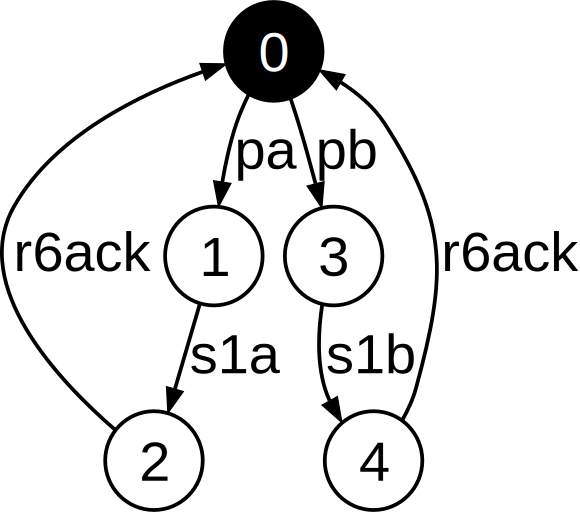
\includegraphics[scale=0.2]{prop-pres-case-studies/figs/abp-P}
    \caption{Process P}
  \end{subfigure}
  \hfill
  \begin{subfigure}[b]{100pt}
    \centering
    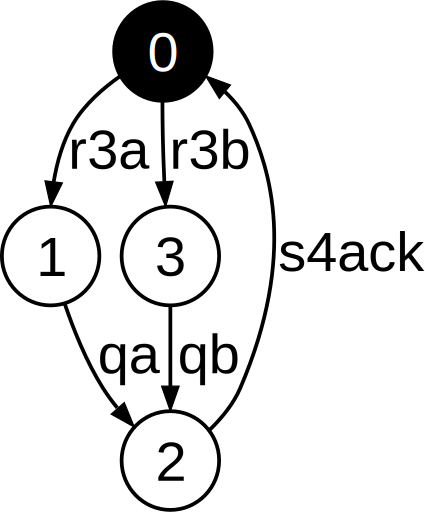
\includegraphics[scale=0.2]{prop-pres-case-studies/figs/abp-Q}
    \caption{Process Q}
  \end{subfigure}
  \hfill
  \begin{subfigure}[b]{130pt}
    \centering
    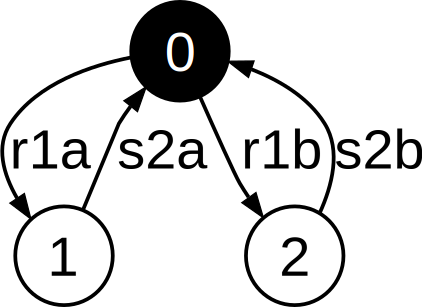
\includegraphics[scale=0.2]{prop-pres-case-studies/figs/abp-B1}
    \caption{Process B1}
  \end{subfigure}
  \\
  \begin{subfigure}[b]{130pt}
    \centering
    \includegraphics[scale=0.2]{prop-pres-case-studies/figs/abp-B2}
    \caption{Process B2}
  \end{subfigure}
  \hfill
  \begin{subfigure}[b]{100pt}
    \centering
    \includegraphics[scale=0.2]{prop-pres-case-studies/figs/abp-B3}
    \caption{Process B3}
  \end{subfigure}
  \hfill
  \begin{subfigure}[b]{130pt}
    \centering
    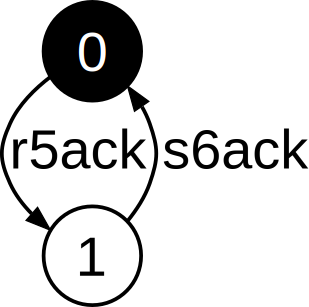
\includegraphics[scale=0.2]{prop-pres-case-studies/figs/abp-B4}
    \caption{Process B4}
  \end{subfigure}
  \caption{Process LTSs of the components shown in Figure~\ref{fig:prop-pres-case-studies:abp-abstract}}
  \label{fig:lts-transformation:abp_processes}
\end{figure}

Figure~\ref{fig:prop-pres-case-studies:abp-rules} shows two transformation rules that replace two of the buffers by two processes that implement the alternating bit protocol.
The alternating bit is encoded by the added suffixes ``t'' and ``f'' in the transition labels.
To make the rule system synchronization uniform regarding the synchronization rules of the system, there are also transformation rules for the other processes that only perform some simple renaming, for instance to rename \action{pa} to \action{pa'}.
Lossy communication is simulated by adding two versions of the synchronization rules that specify how the actions representing communication between components~\Component{B1} and~\Component{B2} synchronize.
One version specifies that a pair of such actions synchronize and lead to successful communication, and the other specifies that an action that represents sending a message can also be performed independently.
The erroneous version of this transformation mentioned in Section~\ref{sec:lts-transformation:experiments} misses the loops on states~$\it{ix}$ and~$\it{xiv}$ that represent the reception of messages with the wrong bit.

\begin{figure}[hbt]
\centering
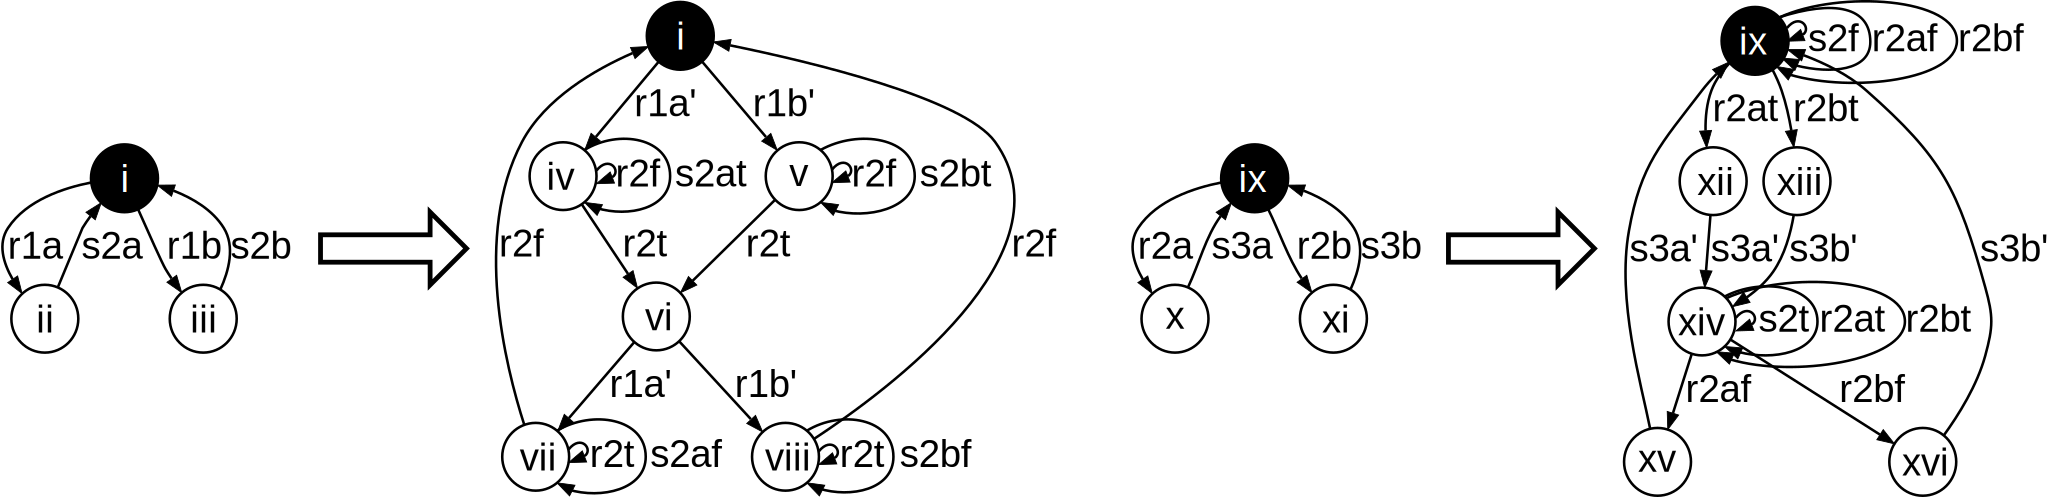
\includegraphics[width=1.0\linewidth]{prop-pres-case-studies/figs/abp-rules}
\caption{Two transformation rules that replace buffers}
\label{fig:prop-pres-case-studies:abp-rules}
\end{figure}

%%%Applying this transformation to the five concurrent communicating systems and adding appropriate synchronization rules in the obtained network of LTSs leads to an explosion of the state-space and thus to a large exploration time.
%%%Checking whether these transformation rules preserve properties, however, takes very little time.
